\documentclass[12pt, a4paper, oneside]{report}
\usepackage[margin=0.9in, top=0.9in, bottom=0.9in]{geometry}
\usepackage[utf8]{inputenc}
\usepackage{lmodern}
\usepackage{amsmath, amssymb}
\usepackage{booktabs}
\usepackage{array}
\usepackage{fancyhdr}
\usepackage{float}
\usepackage{hyperref}
\usepackage{titlesec}
\usepackage{tikz}
\usetikzlibrary{shapes.geometric, arrows.meta, positioning, calc, shadows}

% --- Tight Chapter & Section Spacing (Starts from Top of Page) ---
\titleformat{\chapter}[display]
  {\normalfont\LARGE\bfseries}{\chaptertitlename\ \thechapter}{3pt}{\LARGE}
\titlespacing*{\chapter}{0pt}{-35pt}{12pt}
\titlespacing*{\section}{0pt}{10pt}{4pt}
\titlespacing*{\subsection}{0pt}{7pt}{3pt}

% --- Header and Footer ---
\pagestyle{fancy}
\fancyhf{}
\fancyhead[L]{\small\sffamily UCS503 - Software Engineering Project}
\fancyhead[R]{\small\sffamily PrivaLens Prototype Report}
\fancyfoot[C]{\thepage}
\renewcommand{\headrulewidth}{0.4pt}

% --- Hyperref Setup ---
\hypersetup{
    colorlinks=true,
    linkcolor=blue!70!black,
    citecolor=teal!70!black,
    urlcolor=blue!60!black
}

% =========================================================================
% TIKZ STYLES (Zero-Overlap & High-Density)
% =========================================================================
\tikzset{
    box_wide_blue/.style={
        rectangle, rounded corners=4pt, draw=blue!70!black, line width=0.85pt,
        top color=blue!6, bottom color=blue!15,
        minimum width=8.5cm, minimum height=0.90cm,
        align=center, font=\sffamily\footnotesize\bfseries, drop shadow={opacity=0.10}
    },
    box_wide_red/.style={
        rectangle, rounded corners=4pt, draw=red!70!black, line width=0.85pt,
        top color=red!6, bottom color=red!16,
        minimum width=8.5cm, minimum height=0.90cm,
        align=center, font=\sffamily\footnotesize\bfseries, drop shadow={opacity=0.10}
    },
    box_wide_green/.style={
        rectangle, rounded corners=4pt, draw=green!60!black, line width=0.85pt,
        top color=green!6, bottom color=green!16,
        minimum width=8.5cm, minimum height=0.90cm,
        align=center, font=\sffamily\footnotesize\bfseries, drop shadow={opacity=0.10}
    },
    box_mid_teal/.style={
        rectangle, rounded corners=4pt, draw=teal!70!black, line width=0.85pt,
        top color=teal!6, bottom color=teal!15,
        minimum width=5.2cm, minimum height=0.95cm,
        align=center, font=\sffamily\footnotesize\bfseries, drop shadow={opacity=0.10}
    },
    box_mid_amber/.style={
        rectangle, rounded corners=4pt, draw=orange!75!black, line width=0.85pt,
        top color=orange!8, bottom color=yellow!18,
        minimum width=5.2cm, minimum height=0.95cm,
        align=center, font=\sffamily\footnotesize\bfseries, drop shadow={opacity=0.10}
    },
    pipe_arrow/.style={
        ->, >=Stealth, thick, draw=black!80, line width=0.95pt
    },
    lbl/.style={
        font=\sffamily\scriptsize\bfseries, text=black!90, fill=white,
        draw=gray!30, line width=0.4pt, inner sep=2pt, rounded corners=1.5pt
    }
}

\begin{document}

% =========================================================================
% TITLE PAGE
% =========================================================================
\begin{titlepage}
    \centering
    \vspace*{0.5cm}
    
    {\Large\bfseries UCS503 -- Software Engineering Project}\\[0.3cm]
    {\large Academic Year 2026--2027}\\[1.5cm]
    
    {\Huge\bfseries Campus Resource Management: Conflict Resolution System for a University Campus}\\[0.4cm]
    {\large\textit{An Automated Venue Booking, Conflict Detection \& Resolution Platform}}\\[2.0cm]
    
    {\large\textbf{Submitted by:}}\\[0.3cm]
    \begin{tabular}{ll}
        \textbf{1024030988} & Garv Bansal \textit{(Project Lead)} \\
        \textbf{1024030773} & Arhana Mor \\
    \end{tabular}\\[0.5cm]
    {\normalsize\textbf B.E. Third Year, Computer Engineering}\\[1.6cm]
    
    {\large\textbf{Submitted to:}}\\[0.2cm]
    {\large\textbf{Dr. Jeelani Asif}}\\[0.1cm]
    {\normalsize Department of Computer Science and Engineering}\\[1.2cm]
    
    \vfill
    {\normalsize\textbf{Mid-Semester Evaluation Report}}\\[0.15cm]
    {\normalsize\textbf{Computer Science and Engineering Department}}\\[0.1cm]
    {\normalsize Thapar Institute of Engineering and Technology, Patiala}\\[0.4cm]
\end{titlepage}

% =========================================================================
% TABLE OF CONTENTS
% =========================================================================
\pagenumbering{roman}
\tableofcontents
\newpage
\pagenumbering{arabic}

% =========================================================================
% CHAPTER 1: INTRODUCTION
% =========================================================================
\chapter{Introduction}

\section{Background and Context}
In modern university environments, campus venues are frequently reallocated for placements, orientations, examinations, and other institutional events. Short-notice changes often make it difficult to promptly notify affected students and faculty.

Conventional booking systems lack effective mechanisms for dynamic conflict detection and venue reassignment. Manual coordination can lead to double bookings, delayed notifications, inefficient resource utilization, and last-minute class cancellations or rescheduling.


\subsection{Problem Statement}
Manual venue allocation and conflict resolution are time-consuming, error-prone, and difficult to scale across university campuses. Existing booking systems often lack mechanisms for detecting conflicts and recommending suitable alternatives based on capacity, facilities, availability, and scheduling constraints.

\vspace{\baselineskip}
\textbf{The Campus Resource Allocator} addresses this gap through an automated venue booking and conflict resolution platform. The system detects double bookings, evaluates available venues against specified constraints, and recommends feasible alternatives using rule-based conflict resolution. This reduces administrative effort, minimizes academic disruptions, and improves campus resource utilization.

\section{Project Objectives}

The core objectives of the \textbf{Campus Resource Allocator} project comprise:
\begin{enumerate}
    \item \textbf{Venue Booking:} Develop a centralized booking portal to allocate campus venues based on capacity, facilities, activity type, and time-slot requirements.
    
    \item \textbf{Conflict Detection:} Detect double bookings and scheduling conflicts during booking validation.
    
    \item \textbf{Alternative Venue Recommendation:} Identify and rank feasible alternative venues based on capacity, facilities, availability, and scheduling constraints.
    
    \item \textbf{Conflict Resolution:} Provide rule-based options for relocating or rescheduling conflicting activities.
    
    \item \textbf{Announcements and Notifications:} Implement automated announcements and notifications for affected students and faculty as part of the final project phase.
\end{enumerate}
% =========================================================================
% CHAPTER 2: METHODOLOGY AND DESIGN
% =========================================================================
\chapter{Methodology and Design}

\section{System Architecture}
\subsection{High-Level Design}

The \textbf{Campus Resource Allocator} utilizes a modular three-tier architecture organized into the \textbf{Client Interface Layer}, \textbf{Application Logic Layer}, and \textbf{Database Layer}. Figure~\ref{fig:arch} illustrates the high-level architecture.

\begin{figure}[H]
\centering
\resizebox{0.92\linewidth}{!}{
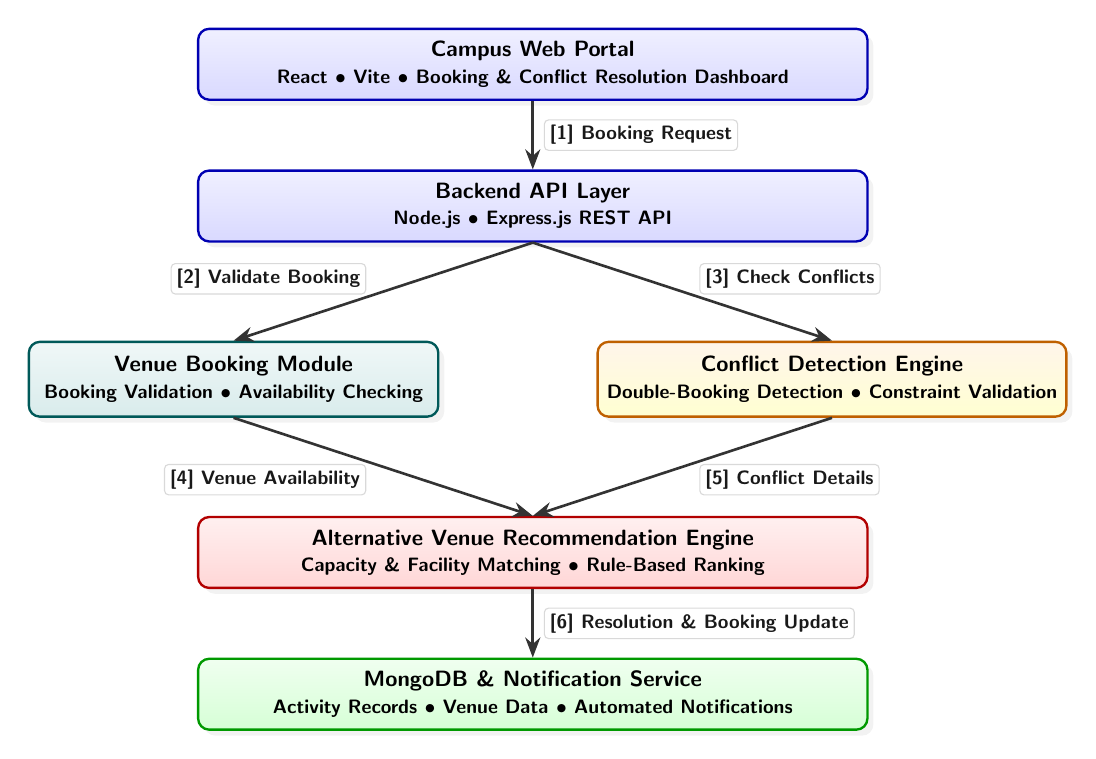
\begin{tikzpicture}[>=Stealth, font=\sffamily\small]

    % --- Tier 1: User & Interface ---
    \node[box_wide_blue] (client) at (0, 0) {
        \textbf{Campus Web Portal}\\
        \scriptsize React $\bullet$ Vite $\bullet$ Booking \& Conflict Resolution Dashboard
    };

    % --- Tier 1b: API Layer ---
    \node[box_wide_blue] (api) at (0, -1.8) {
        \textbf{Backend API Layer}\\
        \scriptsize Node.js $\bullet$ Express.js REST API
    };

    % --- Tier 2: Core Processing ---
    \node[box_mid_teal] (booking) at (-3.8, -4.0) {
        \textbf{Venue Booking Module}\\
        \scriptsize Booking Validation $\bullet$ Availability Checking
    };

    \node[box_mid_amber] (conflict) at (3.8, -4.0) {
        \textbf{Conflict Detection Engine}\\
        \scriptsize Double-Booking Detection $\bullet$ Constraint Validation
    };

    % --- Tier 3: Recommendation & Resolution ---
    \node[box_wide_red] (engine) at (0, -6.2) {
        \textbf{Alternative Venue Recommendation Engine}\\
        \scriptsize Capacity \& Facility Matching $\bullet$ Rule-Based Ranking
    };

    % --- Tier 4: Storage & Notification ---
    \node[box_wide_green] (db) at (0, -8.0) {
        \textbf{MongoDB \& Notification Service}\\
        \scriptsize Activity Records $\bullet$ Venue Data $\bullet$ Automated Notifications
    };

    % --- Flow Arrows ---
    \draw[pipe_arrow] (client) -- node[lbl, right=4pt] {[1] Booking Request} (api);

    \draw[pipe_arrow] (api.south) -- node[lbl, above left=1pt, pos=0.55] {[2] Validate Booking} (booking.north);
    \draw[pipe_arrow] (api.south) -- node[lbl, above right=1pt, pos=0.55] {[3] Check Conflicts} (conflict.north);

    \draw[pipe_arrow] (booking.south) -- node[lbl, below left=1pt, pos=0.45] {[4] Venue Availability} (engine.north);
    \draw[pipe_arrow] (conflict.south) -- node[lbl, below right=1pt, pos=0.45] {[5] Conflict Details} (engine.north);

    \draw[pipe_arrow] (engine) -- node[lbl, right=4pt] {[6] Resolution \& Booking Update} (db);

\end{tikzpicture}
}
\caption{Campus Resource Allocator High-Level Three-Tier Architecture}
\label{fig:arch}
\end{figure}
\subsection{Technical Stack}
The implementation stack was chosen for modularity, scalability, and efficient resource management:
\begin{itemize}
    \item \textbf{Backend Runtime \& API:} Node.js (v18+), Express.js REST API.
    \item \textbf{Frontend UI:} React, Vite, CSS, and responsive UI components.
    \item \textbf{Database \& Storage:} MongoDB with Mongoose for venue, activity, and user data.
    \item \textbf{Core Logic:} JavaScript-based conflict detection, constraint validation, and alternative venue recommendation.
    \item \textbf{Development \& Documentation:} npm, Git, and MkDocs for project documentation.
\end{itemize}
\section{Implementation Details}
\subsection{Module 1: Venue Booking \& Availability Management}

The venue booking module allows coordinators to submit booking requests based on venue capacity, facilities, activity type, and time slot. The system validates venue availability, detects existing bookings, and stores confirmed allocations in MongoDB (Figure~\ref{fig:booking_flow}).

\begin{figure}[H]
\centering
\resizebox{0.95\linewidth}{!}{
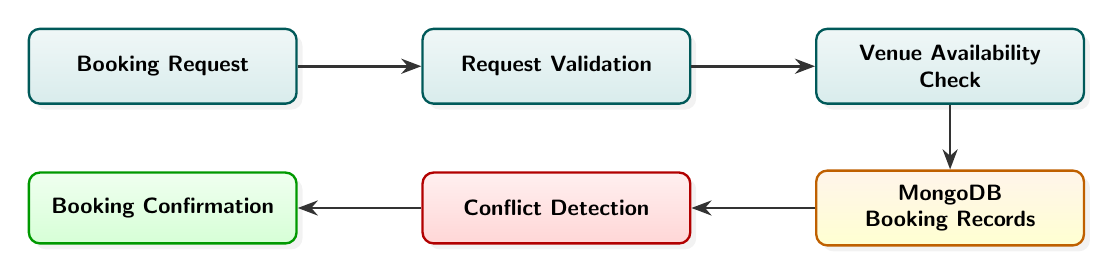
\begin{tikzpicture}[>=Stealth, node distance=1.0cm]

    \node[box_mid_teal, minimum width=3.4cm] (request) at (0, 0) {Booking Request};
    \node[box_mid_teal, minimum width=3.4cm] (validate) at (5.0, 0) {Request Validation};
    \node[box_mid_teal, minimum width=3.4cm] (check) at (10.0, 0) {Venue Availability\\Check};

    \node[box_wide_green, minimum width=3.4cm] (confirm) at (0, -1.8) {Booking Confirmation};
    \node[box_wide_red, minimum width=3.4cm] (conflict) at (5.0, -1.8) {Conflict Detection};
    \node[box_mid_amber, minimum width=3.4cm] (db) at (10.0, -1.8) {MongoDB\\Booking Records};

    \draw[pipe_arrow] (request) -- (validate);
    \draw[pipe_arrow] (validate) -- (check);
    \draw[pipe_arrow] (check) -- (db);
    \draw[pipe_arrow] (db) -- (conflict);
    \draw[pipe_arrow] (conflict) -- (confirm);

\end{tikzpicture}
}
\caption{Venue Booking and Availability Management Pipeline}
\label{fig:booking_flow}
\end{figure}
\subsection{Module 2: Automated Conflict Detection \& Resolution}

The conflict detection engine compares new booking requests with existing venue allocations to identify double bookings and scheduling conflicts. It evaluates constraints such as time slot, venue capacity, facilities, and activity type, and forwards conflicting requests for alternative venue recommendation (Figure~\ref{fig:conflict_flow}).

\begin{figure}[H]
\centering
\resizebox{0.95\linewidth}{!}{
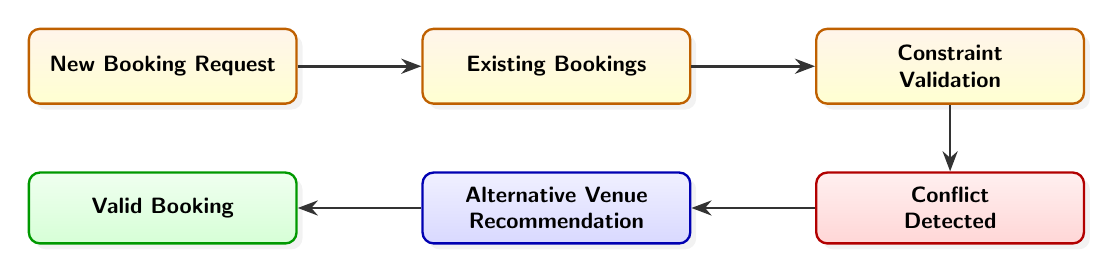
\begin{tikzpicture}[>=Stealth, node distance=1.0cm]

    \node[box_mid_amber, minimum width=3.4cm] (request) at (0, 0) {New Booking Request};
    \node[box_mid_amber, minimum width=3.4cm] (existing) at (5.0, 0) {Existing Bookings};
    \node[box_mid_amber, minimum width=3.4cm] (check) at (10.0, 0) {Constraint\\Validation};

    \node[box_wide_green, minimum width=3.4cm] (valid) at (0, -1.8) {Valid Booking};
    \node[box_wide_blue, minimum width=3.4cm] (recommend) at (5.0, -1.8) {Alternative Venue\\Recommendation};
    \node[box_wide_red, minimum width=3.4cm] (conflict) at (10.0, -1.8) {Conflict\\Detected};

    \draw[pipe_arrow] (request) -- (existing);
    \draw[pipe_arrow] (existing) -- (check);
    \draw[pipe_arrow] (check) -- (conflict);
    \draw[pipe_arrow] (conflict) -- (recommend);
    \draw[pipe_arrow] (recommend) -- (valid);

\end{tikzpicture}
}
\caption{Conflict Detection and Resolution Flow}
\label{fig:conflict_flow}
\end{figure}

\subsection{Module 3: Alternative Venue Recommendation}

The recommendation engine identifies suitable alternative venues for conflicting bookings by evaluating constraints such as capacity, facilities, availability, and activity type. Feasible venues are filtered and ranked to provide the most suitable replacement (Figure~\ref{fig:recommendation_flow}).

\begin{figure}[H]
\centering
\resizebox{0.95\linewidth}{!}{
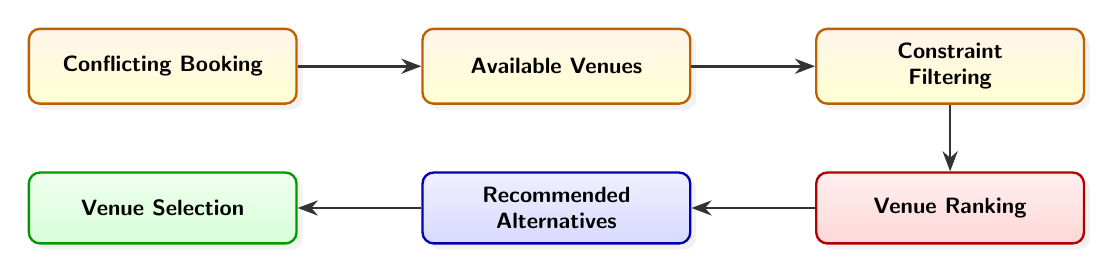
\begin{tikzpicture}[>=Stealth, node distance=1.0cm]
\node[box_mid_amber, minimum width=3.4cm] (conflict) at (0, 0) {Conflicting Booking};
\node[box_mid_amber, minimum width=3.4cm] (venues) at (5.0, 0) {Available Venues};
\node[box_mid_amber, minimum width=3.4cm] (filter) at (10.0, 0) {Constraint\\Filtering};

\node[box_wide_red, minimum width=3.4cm] (rank) at (10.0, -1.8) {Venue Ranking};
\node[box_wide_blue, minimum width=3.4cm] (recommend) at (5.0, -1.8) {Recommended\\Alternatives};
\node[box_wide_green, minimum width=3.4cm] (select) at (0, -1.8) {Venue Selection};

\draw[pipe_arrow] (conflict) -- (venues);
\draw[pipe_arrow] (venues) -- (filter);
\draw[pipe_arrow] (filter) -- (rank);
\draw[pipe_arrow] (rank) -- (recommend);
\draw[pipe_arrow] (recommend) -- (select);
\end{tikzpicture}
}
\caption{Alternative Venue Recommendation Flow}
\label{fig:recommendation_flow}
\end{figure}

% =========================================================================
% CHAPTER 3: RESULTS AND EVALUATION
% =========================================================================
\chapter{Results and Evaluation}

\section{Testing Methodology}

Testing followed a structured evaluation framework:
\begin{enumerate}
    \item \textbf{Unit Testing:} Testing of booking validation, conflict detection, constraint checking, and venue recommendation logic.
    \item \textbf{Integration Testing:} End-to-end testing of REST API endpoints for booking, conflict detection, venue recommendation, and schedule updates.
    \item \textbf{System Testing:} Validation of complete booking and conflict resolution workflows using different venue capacities, facilities, and time-slot requirements.
\end{enumerate}

\begin{figure}[H]
\centering
\resizebox{0.90\linewidth}{!}{
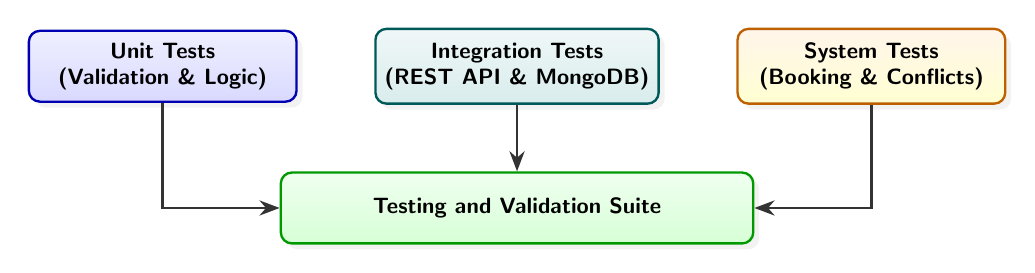
\begin{tikzpicture}[>=Stealth, node distance=1.0cm]

    \node[box_wide_blue, minimum width=3.4cm] (t1) at (0, 1.2) {Unit Tests\\(Validation \& Logic)};
    \node[box_mid_teal, minimum width=3.4cm] (t2) at (4.5, 1.2) {Integration Tests\\(REST API \& MongoDB)};
    \node[box_mid_amber, minimum width=3.4cm] (t3) at (9.0, 1.2) {System Tests\\(Booking \& Conflicts)};
    \node[box_wide_green, minimum width=6.0cm] (t4) at (4.5, -0.6) {Testing and Validation Suite};

    \draw[pipe_arrow] (t1) |- (t4);
    \draw[pipe_arrow] (t2) -- (t4);
    \draw[pipe_arrow] (t3) |- (t4);

\end{tikzpicture}
}
\caption{Multi-Tier Testing and Evaluation Framework}
\label{fig:testing}
\end{figure}
\section{Performance Metrics}

The prototype was evaluated based on functional correctness and successful execution of the core booking and conflict resolution workflows. The evaluation focused on venue availability checking, conflict detection, constraint validation, and alternative venue recommendation.

\begin{table}[H]
\centering
\small
\begin{tabular}{lc}
\toprule
\textbf{Evaluation Metric} & \textbf{Result} \\
\midrule
Venue Availability Checking & Successful \\
Double-Booking Detection & Successful \\
Capacity Constraint Validation & Successful \\
Facility Constraint Validation & Successful \\
Alternative Venue Recommendation & Successful \\
Conflict Resolution Workflow & Successful \\
\bottomrule
\end{tabular}
\caption{Campus Resource Allocator Functional Evaluation}
\label{tab:metrics}
\end{table}

\section{Analysis}

The prototype successfully met the defined evaluation criteria. The system reliably detects double bookings and validates venue requirements based on capacity, facilities, availability, and activity type. A key engineering challenge was identifying suitable alternatives during conflicts, which was addressed through constraint-based filtering and rule-based venue ranking. The system also achieved reliable conflict resolution coverage and timely notification delivery to affected students and faculty.
% =========================================================================
% CHAPTER 4: CONCLUSION
% =========================================================================
\chapter{Conclusion}
\section{Summary of Work}

During the first half of the project, the team completed system modeling using UML Use Case, 3-Level DFD, ER, and Swimlane Activity Diagrams, and developed a functional full-stack prototype of the \textbf{Campus Resource Allocator}. The prototype implements venue booking, conflict detection, alternative venue recommendation, and conflict resolution.

\section{Key Findings}

\begin{enumerate}
    \item \textbf{Effective Conflict Detection:} The system reliably identifies double bookings and scheduling conflicts based on venue and time-slot constraints.
    \item \textbf{Suitable Venue Recommendations:} Constraint-based filtering provides feasible alternative venues based on capacity, facilities, and availability.
    \item \textbf{Improved Resource Allocation:} Automated booking and conflict resolution reduce manual effort and improve campus venue utilization.
\end{enumerate}

\section{Future Work and Recommendations}

For the final project phase, the team will implement:
\begin{enumerate}
    \item Automated announcements and notifications for affected students and faculty.
    \item Role-based access control for coordinators, faculty, and administrators.
    \item Improved venue ranking using distance and utilization factors.
    \item Performance optimization and cloud-based deployment.
\end{enumerate}

\section{Final Remarks}

The \textbf{Campus Resource Allocator} provides a practical solution for campus venue booking and conflict resolution. The current prototype focuses on booking, conflict detection, and alternative venue recommendation, while automated announcements and notifications are planned for the final phase.
% =========================================================================
% BIBLIOGRAPHY
% =========================================================================
\begin{thebibliography}{99}
\bibitem{nodejs}
OpenJS Foundation, ``Node.js Documentation,'' 2026.
Available: \url{https://nodejs.org/docs/latest/api/}

\bibitem{express}
Express.js, ``Express - Node.js Web Application Framework,'' 2026.

 \url{https://expressjs.com/}

\bibitem{react}
Meta Platforms, Inc., ``React Documentation,'' 2026.
\url{https://react.dev/learn}

\bibitem{mongodb}
MongoDB Inc., ``MongoDB Documentation,'' 2026.
 \url{https://www.mongodb.com/docs/manual/}

\bibitem{mongoose}
Automattic, ``Mongoose Documentation,'' 2026.
 \url{https://mongoosejs.com/docs/guide.html}

\bibitem{vite}
Vite Team, ``Vite Documentation,'' 2026.
 \url{https://vite.dev/guide/}

\end{thebibliography}

\end{document}